\documentclass[12pt]{article}

\usepackage{sbc-template}
\usepackage{graphicx,url}
\usepackage[utf8]{inputenc}
\usepackage[brazil]{babel}
% NOTE: the official sbc-template.tex also loads \usepackage[latin1]{inputenc}
% immediately after the utf8 one. That second load silently overrides the
% encoding and would break every accented character in this UTF-8-authored
% file, so it is deliberately NOT repeated here -- this is the one
% intentional deviation from the literal template preamble, kept for
% correctness rather than parity.

\sloppy

\title{Do Diagnóstico ao Reparo: um Pipeline Gerador-Juiz para
  Correção de Vieses Estruturais em Itens de Múltipla Escolha
  Gerados por IA}

\author{Victor Felipe Lourenço da Costa\inst{1}}

\address{Centro de Informática (CIn) -- Universidade Federal de Pernambuco (UFPE)\\
  Recife -- PE -- Brasil
  \email{vflc@cin.ufpe.br}
}

\begin{document}

\maketitle

\begin{abstract}
  This report documents the diagnosis and repair of 239 AI-generated
  multiple-choice educational items rejected on quality grounds (WAPLA 2026,
  Competition 2). An exploratory structural analysis identified four
  quantifiable defects -- position bias, verbosity bias, Bloom's-Taxonomy
  verb/level mismatch, and format-illegal cognitive-level assignment -- and a
  Generator$\leftrightarrow$Judge pipeline, built under a fixed rule set
  derived from a five-module literature review, was used to repair a batch of
  the most severely flawed items. The report documents every deliberate
  deviation from the governing specification, and reports a mid-project
  architectural finding -- a coupling between answer-position assignment and
  content generation -- that was diagnosed and corrected during
  implementation.
\end{abstract}

\begin{resumo}
  Este relatório documenta o diagnóstico e o reparo de 239 questões de
  múltipla escolha geradas por IA e rejeitadas por critérios de qualidade
  (WAPLA 2026, Competição 2). Uma análise exploratória estrutural identificou
  quatro defeitos quantificáveis -- viés de posição, viés de verbosidade,
  incompatibilidade entre verbo e nível na Taxonomia de Bloom, e nível
  cognitivo estruturalmente ilegal para o formato -- e um pipeline
  Generator$\leftrightarrow$Judge, sob um conjunto fixo de regras derivado de
  uma revisão de literatura em cinco módulos, reparou um lote dos itens mais
  defeituosos. O relatório documenta todo desvio deliberado da especificação
  e relata um achado arquitetural -- um acoplamento entre a posição da
  resposta correta e a geração do conteúdo -- diagnosticado e corrigido
  durante a implementação.
\end{resumo}

\section{Introdução}
\label{sec:introducao}

A Competição 2 da WAPLA 2026 (\emph{Quality of AI-Generated Educational
Questions}) parte de um problema concreto e pouco usual em trabalhos sobre
geração automática de itens (\emph{Automated Item Generation}, AIG): em vez
de avaliar itens recém-gerados, o ponto de partida é um conjunto de 239
questões de múltipla escolha \textbf{já geradas por IA e já rejeitadas} por
critérios de qualidade não rotulados explicitamente no
\emph{dataset}\footnote{\texttt{aiboxlab/ai-generated-questions-quality},
  HF, \emph{split} \texttt{data}.}. A tarefa não é apenas
gerar itens novos, mas primeiro \textbf{diagnosticar} por que esses 239 itens
foram rejeitados -- via análise estrutural, não via um rótulo fornecido -- e
então construir um pipeline capaz de \textbf{reparar} um lote desses itens em
questões estruturalmente válidas, sob um conjunto de regras imutável derivado
de uma revisão de literatura em cinco módulos: (1)~pedagogia PBL e Taxonomia
de Bloom \cite{chen2026automated}; (2)~motor AIG sintético e geração de dados
sintéticos preservando privacidade \cite{seedat2025datacentric}; (3)~viés de
juiz LLM e psicometria TRI \cite{zheng2023judging}; (4)~infraestrutura e
Green AI \cite{bai2024beyond}; (5)~rigor de engenharia e artefatos de
especificação \cite{piskala2026specdriven}.

A Seção~\ref{sec:metodologia} descreve a arquitetura implementada e todo
ponto em que diverge de \texttt{spec.md}. A Seção~\ref{sec:descoberta}
relata o achado metodológico central: uma falha arquitetural, não uma
limitação do modelo gerador. A Seção~\ref{sec:resultados} reporta a EDA
e as métricas da execução completa. O notebook completo (EDA e execução
do pipeline) está publicamente disponível no
Kaggle\footnote{URL do notebook Kaggle: \url{https://www.kaggle.com/code/victorflc/notebooke091850abb}.}.

\section{Metodologia}
\label{sec:metodologia}

\subsection{Arquitetura Generator$\leftrightarrow$Judge}

O pipeline (\texttt{WAPLA\_AIG\_Engine.py}) segue a arquitetura
Generator$\leftrightarrow$Judge de \texttt{spec.md} \S4: (i) um
\emph{Generator Agent} reescreve o item a partir do diagnóstico da EDA;
(ii) um \emph{pré-filtro mecânico} verifica posição, verbosidade,
exclusividade e verbo de Bloom antes da chamada ao juiz; (iii) um
\emph{Judge Agent}, modelo arquiteturalmente distinto do gerador,
resolve o item às cegas (\emph{blind-solve}) sobre opções embaralhadas
antes de ver a resposta reivindicada -- decorrelação de viés de posição
(R21/R23). Itens reprovados retornam ao gerador com o motivo da
rejeição; os que esgotam as tentativas seguem para um \emph{pool} de
reserva.

\emph{Nota sobre numeração de regras.} A numeração citada (ex.: R9,
R21, R42) não é sequencial -- deriva de uma especificação interna mais
ampla (\texttt{constitution.md}) da qual este projeto implementa apenas
o subconjunto aplicável à tarefa real; regras fora de escopo permanecem
documentadas como fundamentação para extensões futuras, não como
omissões.

A separação obrigatória entre gerador e juiz (R26) segue a evidência de
viés de autopreferência de \cite{zheng2023judging} (juiz GPT-4 favorece
respostas do próprio GPT-4 em $+10\%$ de taxa de vitória).

\subsection{Desvios Documentados em Relação a \texttt{spec.md}}
\label{sec:desvios}

Seguindo a prática \emph{spec-anchored} \cite{piskala2026specdriven},
quatro desvios deliberados foram registrados: (1)~pré-filtro mecânico em
vez de curador \emph{treinado} (\texttt{spec.md} \S4.2,
\cite{seedat2025datacentric} -- treinar modelos está fora de escopo);
(2)~\emph{single-shuffle} em vez de reordenação 10$\times$
(\texttt{spec.md} \S4.2.1, \cite{pezeshkpour2024large} -- não satisfaz
o piso mínimo de R21); (3)~ausência de checagem de leniência humana/SME
(\texttt{spec.md} \S4.2.1, \cite{kim2025stairaig} -- R24, R33);
(4)~rebaixamento de nível em vez de resposta aberta
(\texttt{spec.md} \S2.5 -- \texttt{determine\_target\_level()} rebaixa
Avaliar/Criar para Analisar, já que o esquema de entrega exige resposta
única).

\subsection{Escolha de Modelos: Afastamento do Princípio Green AI}
\label{sec:green-ai}

\texttt{spec.md} \S5 (\cite{bai2024beyond}) especifica roteamento
sensível a energia/custo entre SLM/MLM/LLM; não implementado. Gerador e
juiz usam modelos gratuitos via Groq
(\texttt{groq/openai/gpt-oss-20b}, \texttt{groq/qwen/qwen3.6-27b}),
satisfazendo a separação de famílias (R26) mas sem medição de energia
ou fronteira de Pareto. \texttt{gpt-oss-20b} é corroborado por
\cite{korthals2026sure} como o mais forte modelo avaliador entre três
testados sob SURE. Afastamento reconhecido do Green AI
\cite{verdecchia2023systematic,shao2026routeandreason}: o prazo tornou
inviável treinar/comparar modelos locais, sem visibilidade das
métricas de eficiência da \S5.4.

\subsection{Medição Real de Energia: Fechando Parcialmente a Lacuna do Green AI}
\label{sec:green-ai-medido}

Execuções locais (\texttt{vllm\_local}, \texttt{cluster-node7} -- cluster
Apuana, CIn-UFPE, GPU A100 80GB) permitem energia real medida no
hardware, não um \emph{proxy} de \emph{tokens}: amostragem de
\texttt{nvidia-smi --query-gpu=power.draw} a cada 2s, integrada pela
regra do trapézio, seguindo \cite{chung2026joules,wang2026systematic}.

\paragraph{Resultados.} Execução completa
(\texttt{phi-4}/\texttt{gpt-oss-20b}, \texttt{cluster-node7}),
$\sim$8.826 amostras a 2s:
\begin{itemize}
  \item Duração: \textbf{5h08min}; potência média \textbf{291,5 W}, pico
    \textbf{408,8 W}
  \item Energia total: \textbf{1,498 kWh}; itens aprovados:
    \textbf{93}/239 ($38{,}9\%$)
  \item \textbf{Energia por item aprovado: 16,1 Wh/item} -- métrica-síntese
    de Green AI desta execução.
\end{itemize}
Mede apenas consumo de GPU (não CPU/rede/infraestrutura compartilhada);
não comparável às execuções via Groq, cuja energia permanece
não-mensurável.

\subsection{Cobertura da Especificação}
\label{sec:cobertura}

A Tabela~\ref{tab:cobertura} consolida, em um único ponto, o status de
cada regra de \texttt{constitution.md} e de cada seção arquitetural de
\texttt{spec.md} frente ao que foi de fato implementado nesta entrega --
substituindo a leitura fragmentada que antes exigia cruzar as três
subseções de divulgação anteriores (\S\ref{sec:desvios},
\S\ref{sec:green-ai} e a limitação de TRI na
Seção~\ref{sec:implicacoes}) com o texto integral de \texttt{spec.md}.

\begin{table}[ht]
\centering
\footnotesize
\begin{tabular}{p{2.6cm}p{6.6cm}p{1.7cm}p{2.9cm}}
\hline
\textbf{Regra(s) / \texttt{spec.md}} & \textbf{Componente} & \textbf{Status} & \textbf{Nota} \\
\hline
R9 (\S II) &
  Formato MCQ ilegal para Avaliar/Criar &
  Implementado &
  \texttt{determine\_target\_level()} rebaixa a Analisar antes da geração
  (Desvio~4, \S\ref{sec:desvios}); confirmado sobre os 100 itens finais:
  zero itens Avaliar/Criar entregues em MCQ. \\
R12--R13 &
  Exclusividade mútua de opções &
  Implementado &
  \texttt{check\_mutual\_exclusivity()} (Jaccard) + exclusividade por
  construção nos formatos templados. \\
R20 (\S IV) / \S4.1, \S4.2 passo~1 &
  Curador CLLM treinado sobre dinâmica de aprendizagem &
  Implementado &
  Pré-filtro mecânico (posição, verbosidade, exclusividade, verbo de
  Bloom) substitui o curador treinado (Desvio~1). \\
R22, R25 &
  Neutralização de viés de verbosidade &
  Implementado &
  \texttt{check\_verbosity()} (CV = 0,35) + auditoria por versão de
  modelo. \\
R31--R34 (\S VII) / \S6.4, \S6.6 &
  Rigor de engenharia, relato estatístico, \emph{spec-anchoring} &
  Implementado &
  Bootstrap/IC em toda a EDA satisfaz R34 integralmente.
  \textbf{Ressalva:} as comparações de calibração do mesmo dia entre
  configurações do \emph{pipeline} ($n=30$ cada, sem \emph{bootstrap})
  não satisfazem R34 por si mesmas -- apenas o \emph{bootstrap} da EDA
  o faz. \\
R37 (\S IX) &
  \emph{Proxy} de energia auditável para inferência \emph{black-box} &
  Implementado &
  Medição real de potência via \texttt{nvidia-smi} a cada 2s +
  integração trapezoidal: $1{,}498$ kWh sobre os 239 itens
  (\S\ref{sec:green-ai-medido}). \\
R38 (\S X) &
  Nenhuma restrição em \emph{prompt} multi-restrição pode ser assumida
  satisfeita pela ordem em que aparece &
  Implementado &
  O pré-filtro mecânico verifica cada restrição de forma independente e
  posterior à geração -- generalização do achado da
  Seção~\ref{sec:descoberta}. \\
R42 (\S XII) &
  Ordem dos campos de \emph{schema}: justificativa antes do veredito &
  Implementado (corrigido v0.9) &
  \texttt{GeneratedItem}/\texttt{JudgeVerdict} e os dois \emph{system
    prompts} corrigidos juntos -- correção só do \emph{schema} era
  insuficiente sob geração em modo JSON. \\
R45 (\S XIII) &
  Controle de comprimento exato via marcadores de contagem regressiva &
  Implementado &
  \emph{Design D}: melhora real de $33{,}3\%$ para $50{,}0\%$ de
  aprovação na calibração isolada, com taxa de malformação de
  marcadores de $77{,}3\%$ (\S\ref{sec:descoberta}). \\
R6--R8 (\S II) / \S2.2, \S2.5 &
  Taxonomia de Bloom, classificador independente &
  Parcial &
  \texttt{check\_bloom\_verb()} é um portão por verbo, não um classificador
  treinado (R8 exige um classificador \emph{independente}, ausente aqui). \\
R10 (\S II) &
  \emph{Template} fixo por nível de Bloom (banco de verbos + regra
  estrutural) &
  Parcial &
  Apenas a metade ``banco de verbos'' tem código; a metade ``regra
  estrutural'' não tem código algum -- todo nível recebe as mesmas
  instruções de estrutura. Ver nota em \texttt{constitution.md} R10. \\
R21, R23, R26 (\S V) / \S4.2.1 passos~1,3,4 &
  Decorrelação de viés de posição; separação arquitetural gerador/juiz &
  Parcial &
  \emph{Single-shuffle} em vez de 10 reordenações (Desvio~2); não
  satisfaz o piso de R21 no modo padrão. \\
\S2.6 &
  Detector de \emph{item-writing flaws} (31-guideline/19-flaw) &
  Parcial &
  Pré-filtro mecânico aproxima o papel do detector, mas não implementa
  a taxonomia completa de 19 falhas. \\
\S3 &
  \emph{Checklist} de validade de 16 perguntas &
  Parcial &
  Subconjunto mecânico coberto; sem disposição final logada como
  \emph{gate} formal. \\
\S4.3 &
  Lógica de roteamento; \emph{flag} de taxa de descarte $>$50\% &
  Parcial &
  \texttt{process\_item()} registra um \emph{warning}, mas não
  interrompe/regenera o lote automaticamente. \\
R24 (\S4.2.1 passo~5) &
  Checagem de leniência contra linha de base humana &
  Desviado &
  Sem revisor humano no \emph{script} automatizado (Desvio~3). \\
R41 (\S XI) &
  Diversidade/redundância entre itens &
  Auditoria pós-hoc &
  \texttt{tools/diversity\_check\_r41.py}, não integrado à seleção
  (\S\ref{sec:diversidade}). \\
R1--R5, R11, R14--R19, R27--R30, R35--R36, R39--R40,
R43--R44 / \S5, \S6, \S2.7--2.9 &
  Blueprint PBL; TRI; dados sintéticos reais; rubricas; consistência
  multi-passagem do juiz; decodificação restrita; Green AI; correção a
  estudantes &
  Fora de escopo &
  Fora do escopo real da tarefa (reparo de itens existentes). Detalhe
  regra a regra no Amendment Log de \texttt{constitution.md}. \\
\hline
\end{tabular}
\caption{Cobertura da especificação: toda regra de \texttt{constitution.md}
  e seção arquitetural de \texttt{spec.md}, frente ao que foi de fato
  implementado nesta entrega.}
\label{tab:cobertura}
\end{table}

\section{Descoberta Metodológica Central: Acoplamento entre Posição e
  Conteúdo}
\label{sec:descoberta}

Durante a calibração, a taxa de aprovação observada foi mais baixa que o
esperado. A investigação revelou uma \textbf{falha arquitetural de
  design de prompt, não uma limitação de capacidade do modelo gerador}:
na primeira versão do pipeline, a letra-alvo balanceada
(\texttt{TARGET\_LETTER}, R21) era injetada no prompt do gerador
\emph{antes} de o conteúdo existir, forçando o modelo a competir entre
correção posicional e correção de conteúdo numa única chamada. Inspeção
manual de casos em que o \emph{blind-solve} do juiz discordava da letra
reivindicada (itens 63, 392, 457) confirmou o padrão: o gerador
satisfazia a posição de forma confiável, mas nem sempre garantia que o
conteúdo ali colocado fosse genuinamente correto.

\textbf{Correção:} o gerador passou a escrever sempre a resposta correta
como \texttt{option\_a}, concentrando-se apenas em garantir correção de
conteúdo; o reposicionamento para a letra-alvo (R21) é aplicado
\textbf{mecanicamente, depois da geração} -- uma troca de \emph{strings}
sobre valores já corretos (\texttt{apply\_position\_shuffle()}), não
mais uma restrição durante a geração. Confirmado em escala
(Seção~\ref{sec:metricas-run}): sobre 749 \emph{attempts}, $9{,}1\%$
tiveram o juiz discordando da letra alegada, mas essas discordâncias
são hoje, por construção, de \textbf{conteúdo}, nunca de
\textbf{posição} -- a atribuição de posição é uma operação
determinística pós-geração, estruturalmente incapaz de reproduzir a
falha original.

\subsection{Um Segundo Ciclo: Controle de Comprimento como Método
  Científico}
\label{sec:segundo-ciclo}

Um segundo achado arquitetural seguiu a mesma lógica científica:
hipótese, teste, refutação, causa-raiz, nova hipótese, confirmação
parcial. \textbf{R42:} \cite{tam2024speak} mostram que a ordem de campos
do \emph{schema} (resposta antes de justificativa) causa colapso de
acurácia (até $86{,}51\%\to23{,}44\%$ no GSM8K); a mesma inversão foi
encontrada e corrigida em \texttt{WAPLA\_AIG\_Engine.py}. \textbf{Design
  C:} testado, refutado -- um alvo numérico de comprimento por item não
alterou aprovação nem extremo de comprimento, pois
\texttt{check\_verbosity()} testa apenas se a opção correta é o extremo
estrito (\emph{ranking}), não um valor absoluto. \textbf{Design D:}
\cite{xie2026length} propõem CAPEL (marcadores de contagem regressiva
visíveis); adotado aqui, aprovação subiu de $33{,}3\%$ para $50{,}0\%$
e extremo de comprimento caiu de $82{,}9\%$ para $76{,}7\%$ (confirmado
em escala: $73{,}2\%$ sobre 239 itens), mas $77{,}3\%$ dos
\emph{attempts} tinham marcadores malformados -- a melhoria vem de uma
minoria de execuções corretas, não de o mecanismo ser confiável.

\textbf{O piso estrutural de $\sim$$40\%$.} Para cinco valores
independentes, o acaso já torna a opção correta o extremo estrito em
$\sim$$40\%$ dos casos. A taxa \emph{observada}
($82{,}9\%\to73{,}2\%$) fica bem acima desse piso -- há viés real além
do ruído inevitável, e o Design D fechou parte dele. Separar piso
inevitável de viés corrigível é a contribuição metodológica desta
seção.

\section{Resultados}
\label{sec:resultados}

\subsection{Achados Estruturais da Análise Exploratória (EDA)}
\label{sec:eda}

A análise exploratória sobre os 239 itens rejeitados
(\texttt{WAPLA\_EDA.ipynb}) identificou quatro defeitos estruturais
quantificáveis, cada estatística reportada com IC 95\% \emph{bootstrap}
(R34, \cite{saleva2025beyond}):

\begin{itemize}
\item \textbf{Viés de posição (R21, R16).} $P(\text{``A''})=80{,}8\%$
  (IC $[75{,}7\%,85{,}8\%]$) contra $20\%$ de chance
  ($\chi^2=558{,}1$, $p=1{,}82\times10^{-119}$).
\item \textbf{Viés de verbosidade (R16, R22).} Opção correta $+2{,}29$
  palavras mais longa em média (IC $[+1{,}74,+2{,}88]$; Wilcoxon
  $p=3{,}64\times10^{-16}$), a mais longa em $49{,}8\%$ dos itens contra
  $20\%$ de chance \cite{haladyna2002review}.
\item \textbf{Incompatibilidade com Bloom (R6--R11).} $96$ itens
  ($40{,}2\%$) sem verbo canônico de nível algum no item; entre os
  demais, $68{,}2\%$ de incompatibilidade entre nível declarado e
  inferido \cite{haladyna2013developing}.
\item \textbf{Formato MCQ estruturalmente ilegal.} $172$ itens
  ($72{,}0\%$) declarados Avaliar/Criar mas entregues em múltipla
  escolha de resposta única -- ilegal sob R9 (Avaliar é o caso mais
  limítrofe dos dois; ver nota de escopo em \texttt{constitution.md}).
\end{itemize}

Em média, cada item carrega $2{,}27$ desses quatro sinalizadores
simultaneamente; apenas $4$ itens ($1{,}7\%$) não apresentam nenhum --
rejeitados por razões fora do escopo desses \emph{checks} (ex.: erro
factual, ambiguidade detectável apenas por humano).

Execução completa do \emph{pool} de 239 candidatos
(\texttt{phi-4}/\texttt{gpt-oss-20b}, \texttt{cluster-node7}) atingiu a
meta de $100$ itens em duas passagens ($93/239=38{,}9\%$; $+10/40=25{,}0\%$
sobre o subconjunto mais difícil do \emph{pool} de reserva), com energia
real medida (Seção~\ref{sec:green-ai-medido}) de $1{,}498$ kWh ($16{,}1$
Wh/item aprovado).\label{sec:metricas-run} Uma auditoria
pós-entrega,\label{sec:auditoria-qwen} reexecutando o \emph{blind-solve}
com um segundo juiz (\texttt{qwen3.6-27b}) sobre o lote entregue,
sinalizou $27\%$ dos itens com \texttt{bloom\_alignment\_ok=False} (até
$50\%$ falhando algum critério) -- \emph{stems} usando o verbo declarado
apenas retoricamente, sem exigir análise real; a correção
(\texttt{determine\_target\_level()}, $23$ itens rebaixados de
``Analisar'' para ``Compreender'', $43$ regenerados no total) mudou a
composição de $100$ Analisar para $70$/$22$/$8$
(Analisar/Compreender/Aplicar). O arquivo final entregue é
\texttt{entregavel\_2\_100\_questoes\_qwen\_validated.csv}, com
diversidade entre itens (R41,
\texttt{tools/diversity\_check\_r41.py})\label{sec:diversidade} estável
(Self-CosSim $0{,}0607\to0{,}0557$).

\section{Evidências}
\label{sec:evidencias}

As figuras a seguir foram produzidas por \texttt{WAPLA\_EDA.ipynb} e
salvas em \texttt{output/}; não são recriadas aqui, apenas referenciadas, e
seguem o padrão de figura de \cite{rougier2014rules} adotado por
\texttt{spec.md} Seção~6.5 (\emph{colormap} perceptualmente apropriado,
eixos não truncados, legendas autocontidas).

\begin{figure}[ht]
\centering
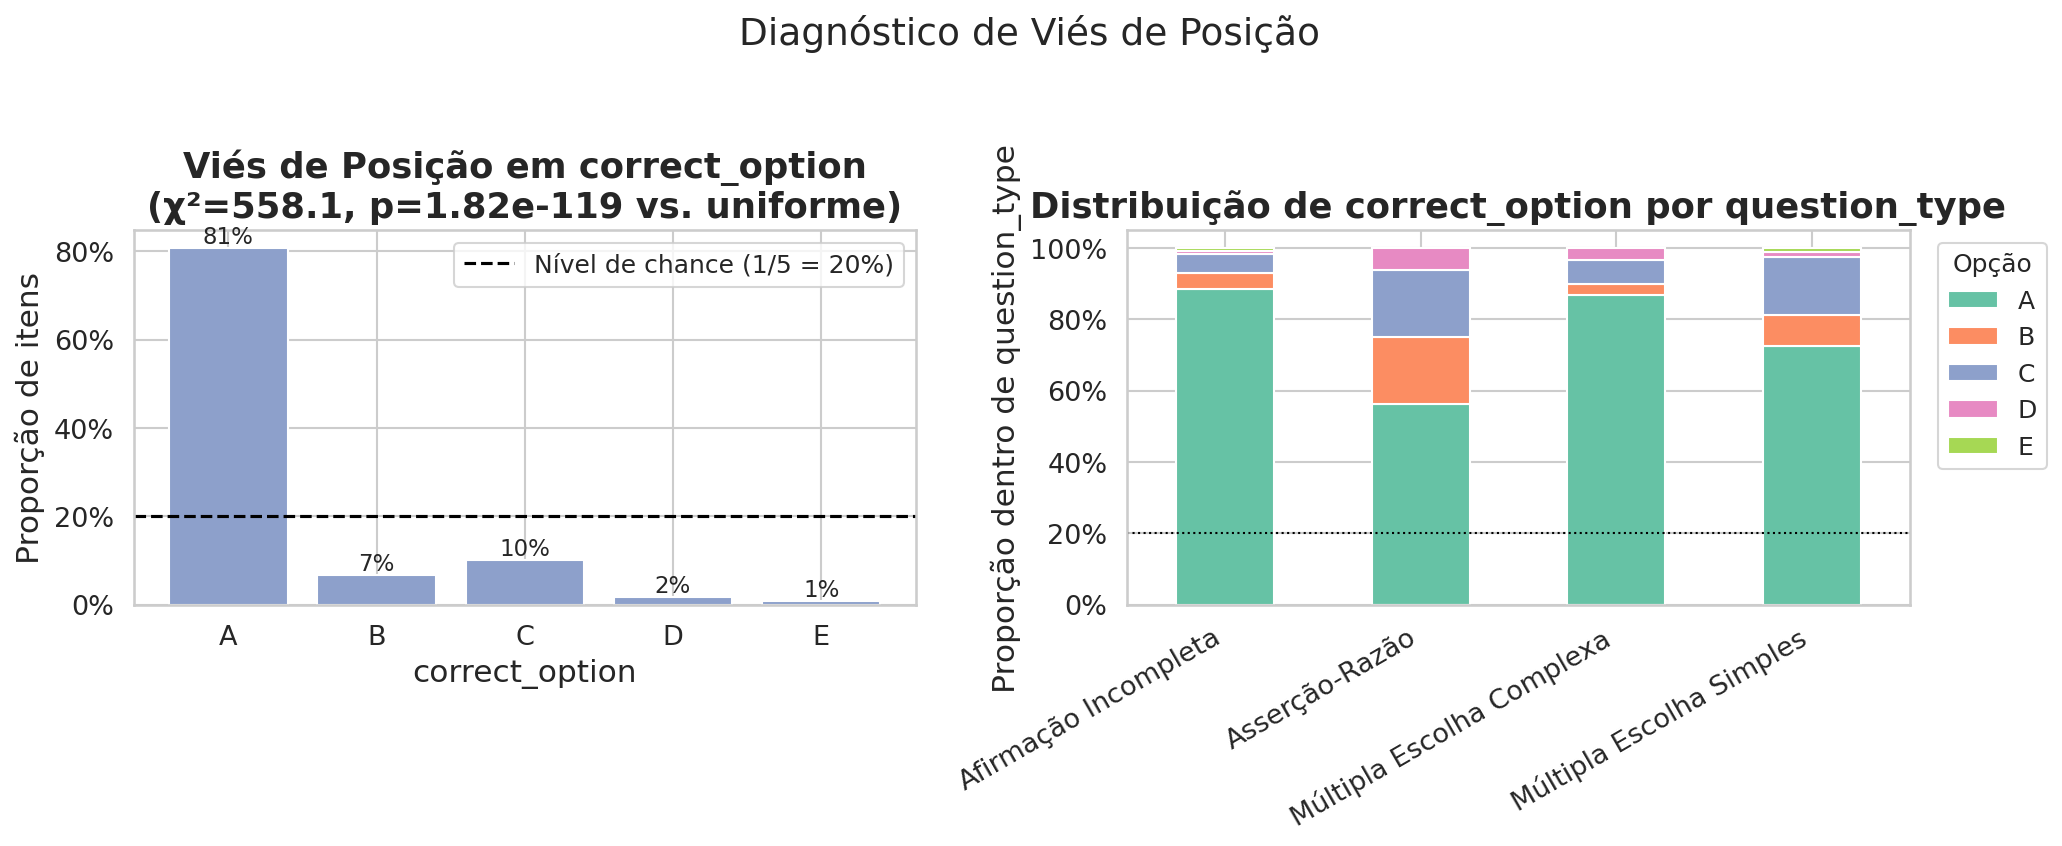
\includegraphics[width=.85\textwidth]{../output/03_position_bias.png}
\caption{Viés de posição: distribuição de \texttt{correct\_option} no corpus
  rejeitado e por \texttt{question\_type}.}
\label{fig:posicao}
\end{figure}

\begin{figure}[ht]
\centering
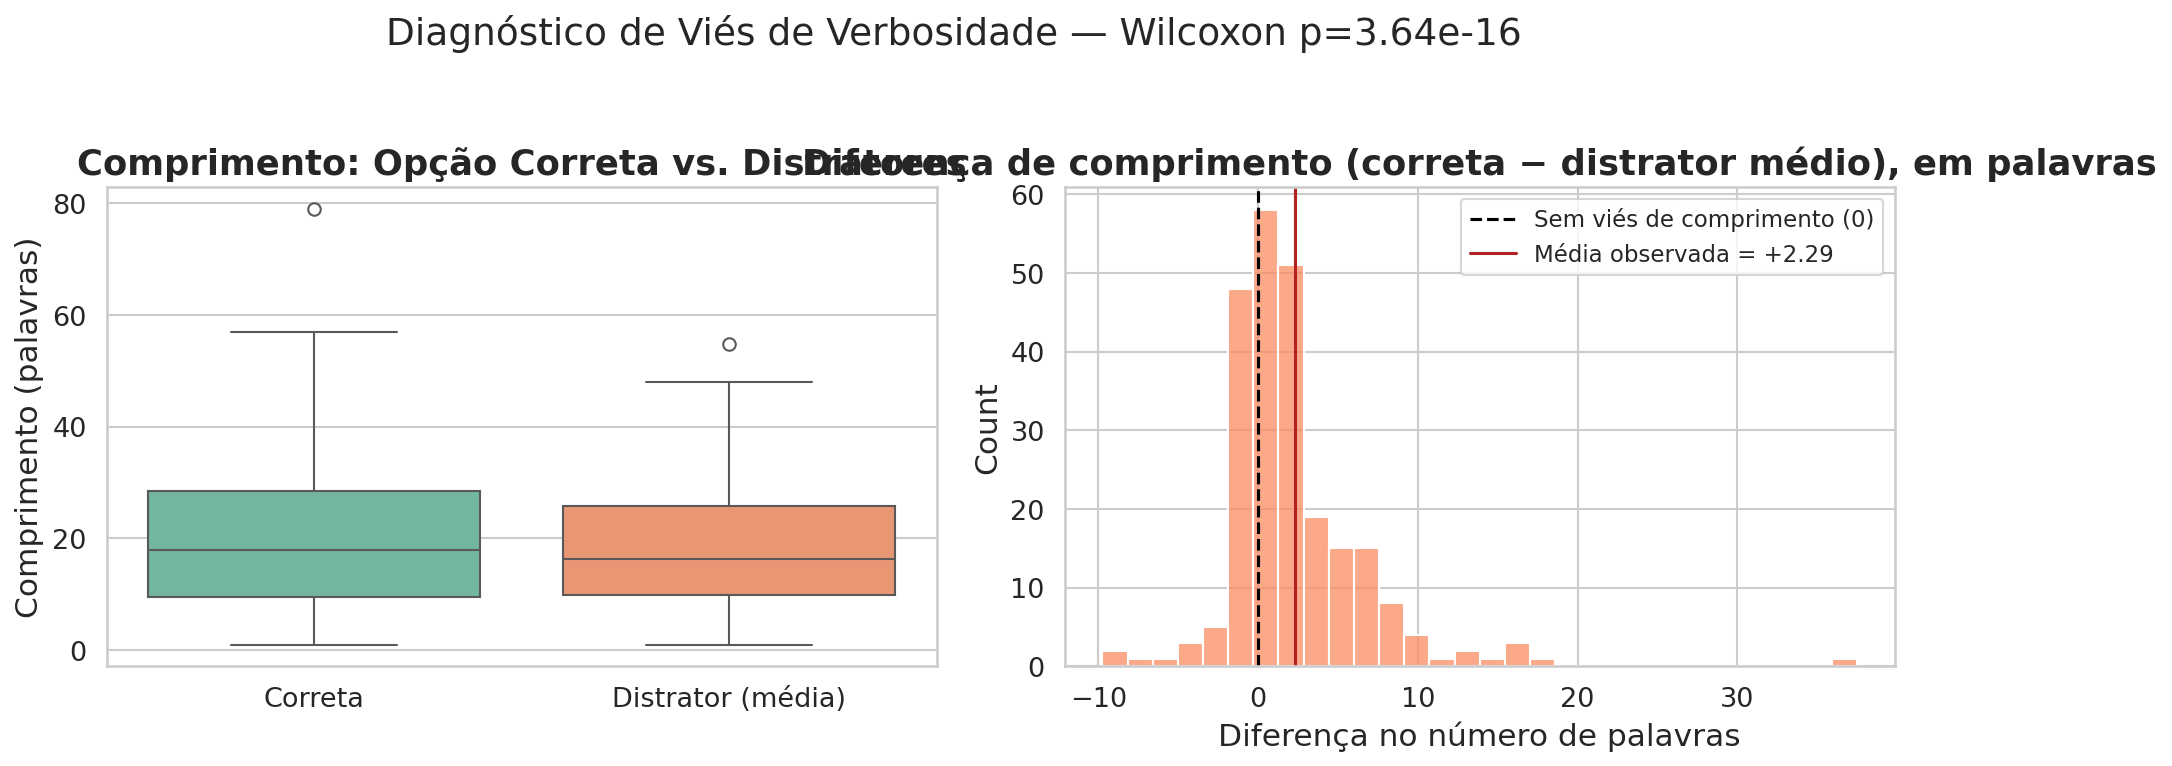
\includegraphics[width=.85\textwidth]{../output/02_verbosity_bias.png}
\caption{Viés de verbosidade: comprimento da opção correta vs.\ distratores
  e distribuição da diferença de comprimento.}
\label{fig:verbosidade}
\end{figure}

% Figura removida para caber no limite de páginas (mantida comentada, não
% excluída, para restauração futura caso o espaço permita).
% \begin{figure}[ht]
% \centering
% 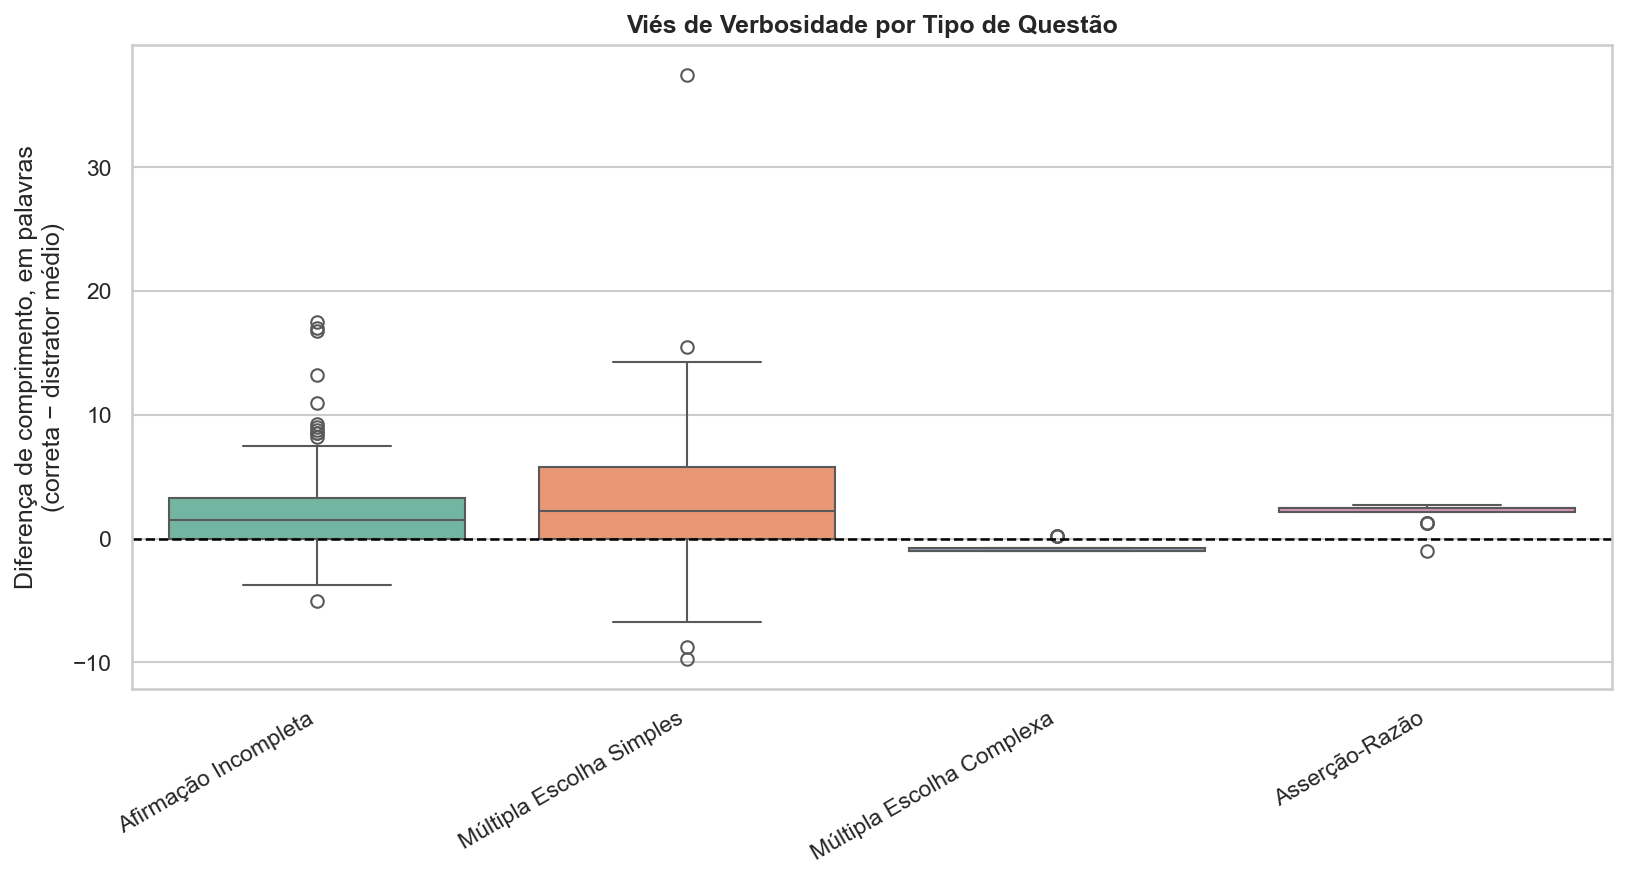
\includegraphics[width=.7\textwidth]{../output/02b_verbosity_bias_by_question_type.png}
% \caption{Viés de verbosidade desagregado por tipo de questão.}
% \label{fig:verbosidade-tipo}
% \end{figure}

\begin{figure}[ht]
\centering
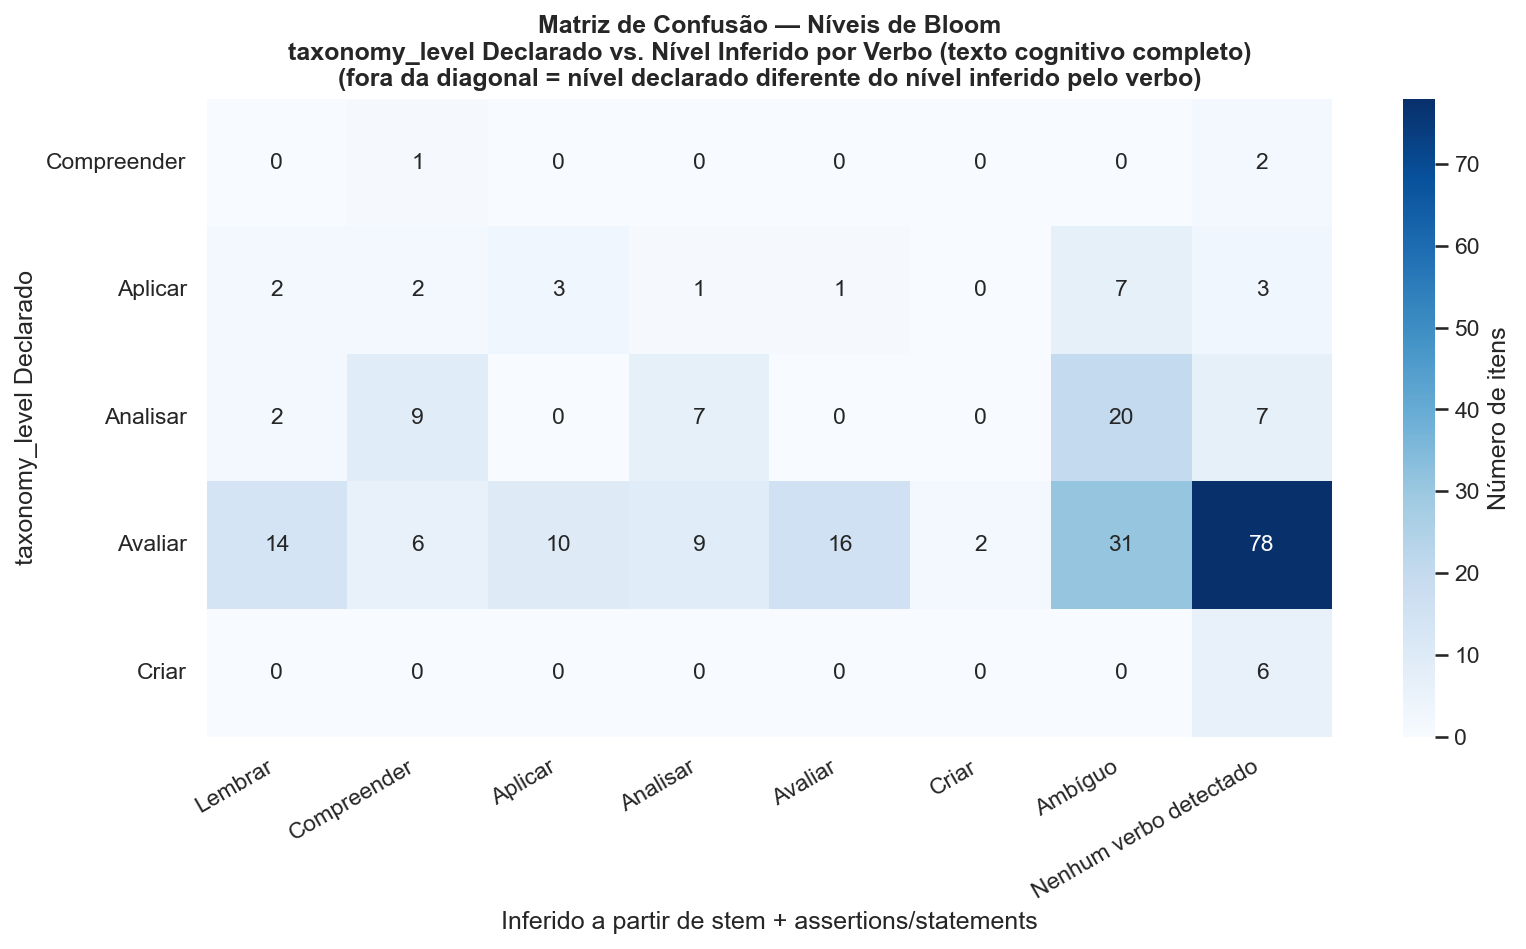
\includegraphics[width=.85\textwidth]{../output/04_bloom_confusion_matrix.png}
\caption{Matriz de confusão entre o nível de Bloom declarado e o nível
  inferido a partir do verbo do texto cognitivo completo.}
\label{fig:bloom}
\end{figure}

% Figura removida para caber no limite de páginas (mantida comentada, não
% excluída, para restauração futura caso o espaço permita).
% \begin{figure}[ht]
% \centering
% 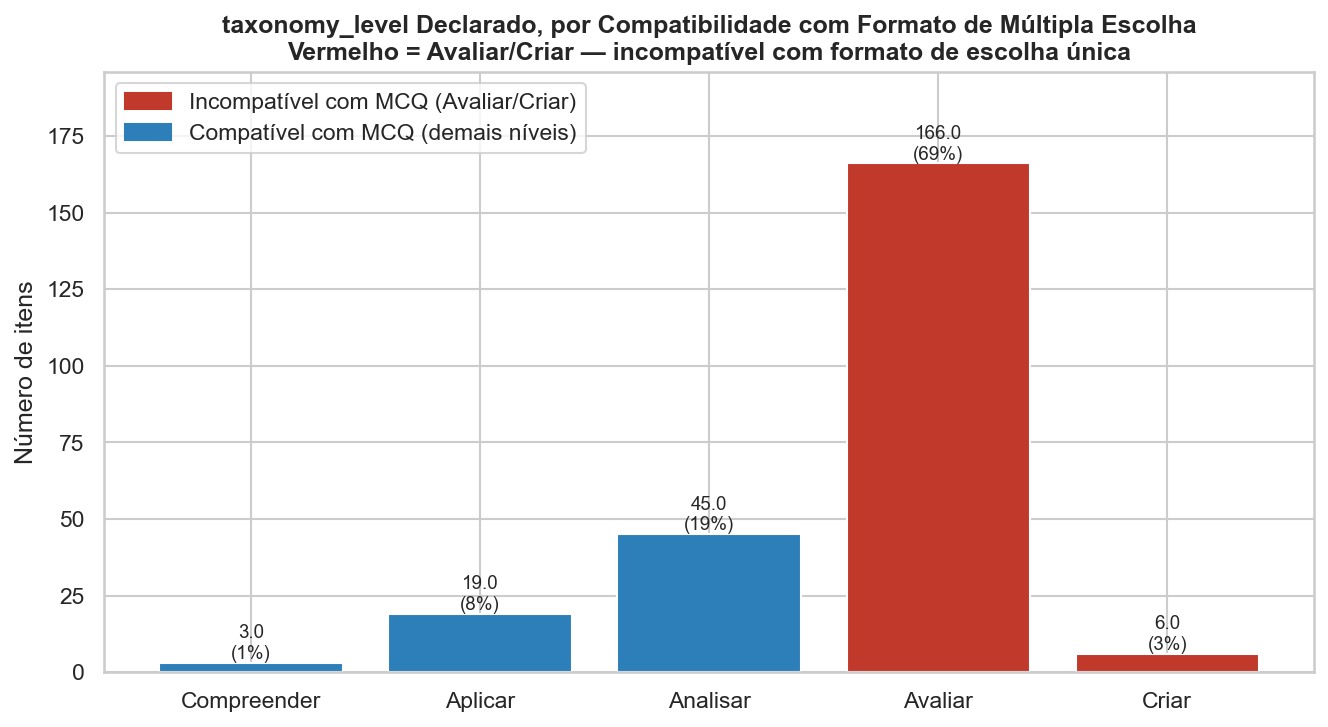
\includegraphics[width=.7\textwidth]{../output/05_r9_format_violation.png}
% \caption{Nível de Bloom declarado, por compatibilidade com o formato de
%   múltipla escolha.}
% \label{fig:r9}
% \end{figure}

% Figura removida para caber no limite de páginas (mantida comentada, não
% excluída, para restauração futura caso o espaço permita).
% \begin{figure}[ht]
% \centering
% 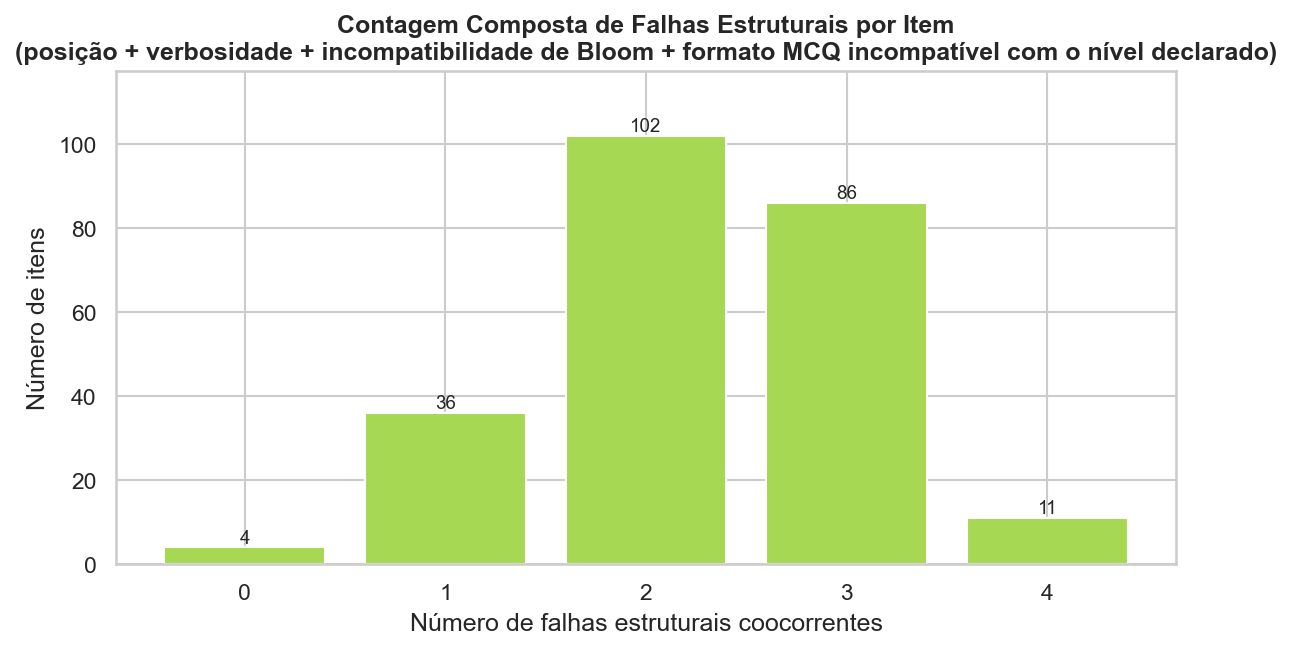
\includegraphics[width=.7\textwidth]{../output/06_composite_flaw_count.png}
% \caption{Contagem composta de falhas estruturais coocorrentes por item.}
% \label{fig:composto}
% \end{figure}

% Figura removida para caber no limite de páginas (mantida comentada, não
% excluída, para restauração futura caso o espaço permita).
% \begin{figure}[ht]
% \centering
% 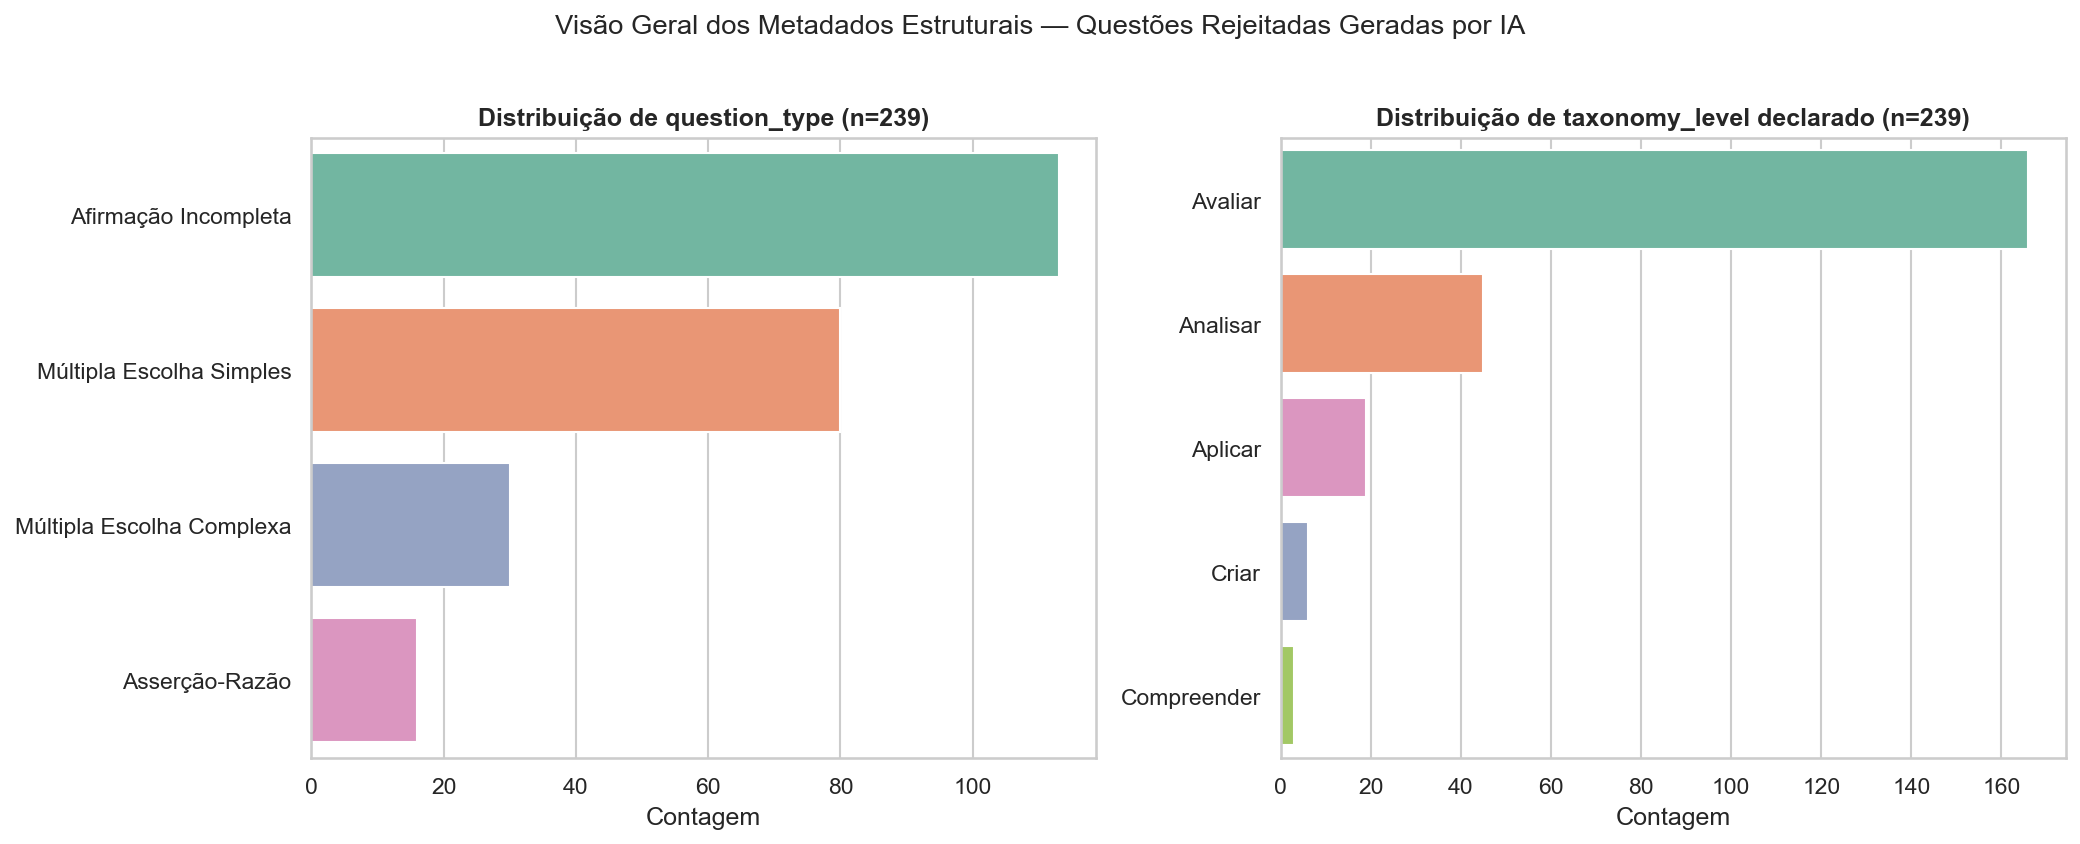
\includegraphics[width=.85\textwidth]{../output/01_overview_distributions.png}
% \caption{Visão geral dos metadados estruturais do corpus rejeitado:
%   distribuição de \texttt{question\_type} e de \texttt{taxonomy\_level}
%   declarado.}
% \label{fig:overview}
% \end{figure}

\section{Implicações para as 100 Questões Finais}
\label{sec:implicacoes}

Cada achado da Seção~\ref{sec:eda} foi operacionalizado no pré-filtro
mecânico: \emph{pool} ordenado por \texttt{structural\_flaw\_count}
decrescente; viés de posição (Figura~\ref{fig:posicao}) via
\texttt{assign\_target\_letters()} (R21) combinado com a correção da
Seção~\ref{sec:descoberta}; viés de verbosidade (Figura~\ref{fig:verbosidade})
via \texttt{check\_verbosity()} (CV$=0{,}35$); incompatibilidade com
Bloom (Figura~\ref{fig:bloom}) via \texttt{check\_bloom\_verb()} (R10);
formato MCQ ilegal via \texttt{determine\_target\_level()}; e
exclusividade mútua intra-item (R12, R13) via
\texttt{check\_mutual\_exclusivity()} (Jaccard) ou por construção nos
formatos templados \cite{bailey2025exploring}.

A lacuna de checagem de leniência humana e o afastamento do princípio
Green AI permanecem como limitações reconhecidas (R33), assim como a
ausência de calibração TRI (\texttt{spec.md} \S4.4, R27) por não existir
ainda um \emph{pool} de respondentes \cite{liu2025leveraging}.

\section*{Uso de IA Generativa}
\label{sec:uso-ia}

Em conformidade com o Código de Conduta para Autores em Publicações da SBC,
declara-se o uso de ferramentas de Inteligência Artificial (IA) Generativa
neste trabalho em dois níveis: (i)~como parte central da metodologia
investigada -- três configurações de modelo distintas, em três momentos
diferentes do projeto, foram usadas como \emph{Generator} e \emph{Judge
  Agents} no próprio pipeline de reparo de itens: os modelos Groq
(\texttt{openai/gpt-oss-20b}, \texttt{qwen/qwen3.6-27b}) na concepção
original da submissão (Seção~\ref{sec:green-ai}); \texttt{phi-4} (gerador)
e \texttt{gpt-oss-20b} (juiz), servidos localmente via
\texttt{vllm\_local}, na execução completa que produziu o lote original
de 100 itens (Seções~\ref{sec:descoberta}--\ref{sec:metricas-run}); e
\texttt{gpt-oss-20b} (gerador) com \texttt{qwen3.6-27b} (juiz),
novamente servidos localmente -- restaurando as identidades de modelo da
concepção original, mas agora com visibilidade direta de hardware --
na auditoria de confiabilidade e correção pós-entrega
(Seção~\ref{sec:auditoria-qwen}) que produziu o arquivo final
efetivamente entregue; e (ii)~como assistente de
escrita e revisão na elaboração deste relatório e do código do pipeline
(Claude, Anthropic). Nenhuma ferramenta de IA é listada como autora; a
responsabilidade pelo conteúdo é dos autores humanos.

\bibliographystyle{sbc}
\bibliography{relatorio_tecnico}

\end{document}
